\documentclass[10.5pt,compsoc]{CjC}
\usepackage{CJKutf8}
%\usepackage{CJK}
\usepackage{graphicx}
\usepackage{footmisc}
\usepackage{subfigure}
\usepackage{url}
\usepackage{multirow}
\usepackage[noadjust]{cite}
\usepackage{amsmath,amsthm}
\usepackage{amssymb,amsfonts}
\usepackage{booktabs}
\usepackage{color}
\usepackage{ccaption}
\usepackage{booktabs}
\usepackage{float}
\usepackage{fancyhdr}
\usepackage{caption}
\usepackage{xcolor,stfloats}
\usepackage{comment}
\setcounter{page}{1}
\graphicspath{{figures/}}
\usepackage{cuted}%flushend,
\usepackage{captionhack}
\usepackage{epstopdf}
%\usepackage{ccmap}
%\CJKtilde
%\usepackage{CJKpunct} 
%\usepackage[lite,subscriptcorrection,slantedGreek,nofontinfo]{mtpro2}

%===============================%

%\firstfootname{ \quad \quad }
\headevenname{\mbox{\quad} \hfill  \mbox{\zihao{-5}{\begin{CJK*}{GBK}{song}¼Æ\quad \quad Ëã\quad \quad »ú\quad \quad ѧ\quad \quad ±¨\end{CJK*}} \hspace {50mm} \mbox{\begin{CJK*}{GBK}{song}2019 Äê\end{CJK*}}}}%
\headoddname{\begin{CJK*}{GBK}{song}? ÆÚ \hfill
×÷ÕßÐÕÃûµÈ£ºÂÛÎÄÌâÄ¿\end{CJK*}}%

%footnote use of *
\renewcommand{\thefootnote}{\fnsymbol{footnote}}
\setcounter{footnote}{0}
\renewcommand\footnotelayout{\zihao{5-}}

\newtheoremstyle{mystyle}{0pt}{0pt}{\normalfont}{1em}{\bf}{}{1em}{}
\theoremstyle{mystyle}
\renewcommand\figurename{figure~}
\renewcommand{\thesubfigure}{(\alph{subfigure})}
\newcommand{\upcite}[1]{\textsuperscript{\cite{#1}}}
\renewcommand{\labelenumi}{(\arabic{enumi})}
\newcommand{\tabincell}[2]{\begin{tabular}{@{}#1@{}}#2\end{tabular}}
\newcommand{\abc}{\color{white}\vrule width 2pt}
\makeatletter
\renewcommand{\@biblabel}[1]{[#1]\hfill}
\makeatother
\setlength\parindent{2em}
%\renewcommand{\hth}{\begin{CJK*}{GBK}{hei}}
%\renewcommand{\htss}{\begin{CJK*}{GBK}{song}}


\begin{document}
\hyphenpenalty=50000
\makeatletter
\newcommand\mysmall{\@setfontsize\mysmall{7}{9.5}}
\newenvironment{tablehere}
  {\def\@captype{table}}

\let\temp\footnote
\renewcommand \footnote[1]{\temp{\zihao{-5}#1}}


\thispagestyle{plain}%
\thispagestyle{empty}%
\pagestyle{CjCheadings}

\begin{table*}[!t]
\vspace {-13mm}
\begin{tabular}{p{168mm}}
\zihao{5-}\begin{CJK*}{GBK}{song}
µÚ??¾í\quad µÚ?ÆÚ \hfill ¼Æ\quad Ëã\quad »ú\quad ѧ\quad ±¨\hfill Vol. ??  No. ?\end{CJK*}\\
\zihao{5-}\begin{CJK*}{GBK}{song}
20??Äê?ÔÂ \hfill CHINESE JOURNAL OF COMPUTERS \hfill ???. 20??\end{CJK*}\\
\hline\\[-4.5mm]
\hline\end{tabular}

\centering
\vspace {11mm}
\begin{CJK}{GBK}{hei}
{\zihao{2} ÌâÄ¿£¨ÖÐÓ¢ÎÄÌâÄ¿Ò»ÖÂ)×ÖÌåΪ2ºÅºÚÌå(È«ÎijýÌرðÉùÃ÷Í⣬ ÍâÎÄͳһÓÃTimes New Roman) }
\end{CJK}
\vskip 5mm

{\zihao{3}\begin{CJK*}{GBK}{fs}
×÷ÕßÃû$^{1)}$\quad  ×÷ÕßÃû$^{2),3)}$ \quad ×÷ÕßÃû$^{3) }$($^*$×ÖÌåΪ3ºÅ·ÂËÎ*×÷Õß)\end{CJK*}}

\vspace {5mm}
\zihao{6}{\begin{CJK*}{GBK}{song}
$^{1)}$(µ¥Î»È«Ãû ²¿ÃÅ(ϵ)È«Ãû, ÊÐ(»òֱϽÊÐ) ¹ú¼ÒÃû ÓÊÕþ±àÂë)
*×ÖÌåΪ6ºÅËÎÌå*µ¥Î»
\end{CJK*}}

\zihao{6}{\begin{CJK*}{GBK}{song}
$^{2)}$(µ¥Î»È«Ãû ²¿ÃÅ(ϵ)È«Ãû, ÊÐ(»òֱϽÊÐ) ¹ú¼ÒÃû
ÓÊÕþ±àÂë)*ÖÐÓ¢Îĵ¥Î»Ãû³Æ¡¢×÷ÕßÐÕÃûÐëÒ»ÖÂ*
\end{CJK*}}

\zihao{6}{\begin{CJK*}{GBK}{song}
$^{3)}$(µ¥Î»È«Ãû ²¿ÃÅ(ϵ)È«Ãû, ÊÐ(»òֱϽÊÐ) ¹ú¼ÒÃû ÓÊÕþ±àÂë)
\end{CJK*}}

\zihao{6}{\begin{CJK*}{GBK}{hei}
ÂÛÎĶ¨¸åºó£¬×÷ÕßÊðÃû¡¢µ¥Î»ÎÞÌØÊâÇé¿ö²»Äܱä¸ü¡£Èô±ä¸ü£¬ÐëÌύǩÕÂÉêÇ룬¹ú¼ÒÃûΪÖйú¿ÉÒÔ²»Ð´£¬Ê¡»á³ÇÊв»Ð´Ê¡µÄÃû³Æ£¬ÆäËû¹ú¼Ò±ØÐëд¹ú¼ÒÃû¡£
\end{CJK*}}

\vskip 5mm
{\centering
\begin{tabular}{p{160mm}}
\zihao{5-}{
\setlength{\baselineskip}{16pt}\selectfont{
\noindent\begin{CJK*}{GBK}{hei}Õª\quad Òª\quad \end{CJK*} \begin{CJK*}{GBK}{song}
*ÖÐÎÄÕªÒªÄÚÈÝÖÃÓÚ´Ë´¦(Ó¢ÎÄÕªÒªÖÐÒªÓÐÕâЩÄÚÈÝ)£¬×ÖÌåΪС5ºÅËÎÌå¡£ÕªÒª¹±Ïײ¿·Ö£¬ÒªÓÐÊý¾ÝÖ§³Ö£¬²»Òª³öÏÖ``...´ó´óÌá¸ß''¡¢``...ÏÔÖø¸ÄÉÆ''µÈÃèÊö£¬ÕýÈ·µÄÃèÊöÊÇ``±È{\ldots}Ìá¸ßX{\%}''¡¢
``ÔÚ{\ldots}ÉϸÄÉÆX{\%}''¡£*ÕªÒª

\end{CJK*}\par}}\\[2mm]

\zihao{5-}{\noindent
\begin{CJK*}{GBK}{hei}¹Ø¼ü´Ê\end{CJK*} \quad \begin{CJK*}{GBK}{song}{*¹Ø¼ü´Ê£¨ÖÐÎĹؼü×ÖÓëÓ¢ÎĹؼü×Ö¶ÔÓ¦ÇÒÒ»Ö£¬Ó¦ÓÐ5-7¸ö¹Ø¼ü´Ê)£»¹Ø¼ü´Ê£»¹Ø¼ü´Ê£»¹Ø¼ü´Ê*  }
\end{CJK*}
}\\[2mm]
\zihao{5-}{\begin{CJK*}{GBK}{hei}ÖÐͼ·¨·ÖÀàºÅ\end{CJK*}	\begin{CJK*}{GBK}{song}
TP\end{CJK*}\rm{\quad \quad \quad     }
\begin{CJK*}{GBK}{hei}DOIºÅ:\end{CJK*}\begin{CJK*}{GBK}{song}
*Ͷ¸åʱ²»ÌṩDOIºÅ\end{CJK*}}
\end{tabular}}

\vskip 7mm

\begin{center}
\zihao{3}{ {\begin{CJK*}{GBK}{hei}Title *£¨ÖÐÓ¢ÎÄÌâÄ¿Ò»ÖÂ)×ÖÌåΪ4ºÅTimes New Roman,¼Ó´Ö* Title\end{CJK*}}}\\
\vspace {5mm}
\zihao{5}{ {\begin{CJK*}{GBK}{hei}NAME Name-Name$^{1)}$ NAME Name$^{2)}$ NAME Name-Name$^{3)}$ *×ÖÌåΪ5ºÅTimes
new Roman*Name\end{CJK*}
}}\\
\vspace {2mm}
\zihao{6}{\begin{CJK*}{GBK}{hei}{$^{1)}$(Department of ****, University, City ZipCode, China) *×ÖÌåΪ6ºÅTimes
new Roman* Depart.Correspond}\end{CJK*}}

\zihao{6}{\begin{CJK*}{GBK}{hei}{$^{2)}$(Department of ****, University, City ZipCode)*Öйú²»Ð´¹ú¼ÒÃû*}\end{CJK*}}

\zihao{6}{\begin{CJK*}{GBK}{hei}{$^{3)}$(Department of ****, University, City ZipCode, country)*Íâ¹úд¹ú¼ÒÃû*}\end{CJK*}}



\end{center}

\begin{tabular}{p{160mm}}
\zihao{5}{
\setlength{\baselineskip}{18pt}\selectfont{
{\bf Abstract}\quad \begin{CJK*}{GBK}{hei}(\textbf{500Ó¢Îĵ¥´Ê£¬ÄÚÈÝ°üº¬ÖÐÎÄÕªÒªµÄÄÚÈÝ}).
×ÖÌåΪTimes new Roman,×ÖºÅ5ºÅ* Abstract\end{CJK*}
\par}}\\

\setlength{\baselineskip}{18pt}\selectfont{
\zihao{5}{\noindent Do not modify the amount of space before and after the artworks. One- or two-column format artworks are preferred. and Tables, create a new break line and paste the resized artworks where desired. Do not modify the amount of space before and after the artworks. One- or two-column format artworks are preferred. All Schemes, Equations, Figures, and Tables should be mentioned in the text consecutively and numbered with Arabic numerals, and appear below where they are mentioned for the first time in the main text. To insert Schemes, Equations, Figures, and Tables, create a new break line and paste the resized artworks where desired. Do not modify the amount of space before and after the artworks. One- or two-column format artworks are preferred.Do not modify the amount of space before and after the artworks. One- or two-column format artworks are preferred. and Tables, create a new break line and paste the resized artworks where desired. Do not modify the amount of space before and after the artworks. One- or two-column format artworks are preferred. All Schemes, Equations, Figures, and Tables should be mentioned in the text consecutively and numbered with Arabic numerals, and appear below where they are mentioned for the first time in the main text.

\vspace {5mm}
{\bf Keywords}\quad \begin{CJK*}{GBK}{hei}ÖÐÎĹؼü×ÖÓëÓ¢ÎĹؼü×Ö¶ÔÓ¦ÇÒÒ»Ö£¬\textbf{²»ÒªÓÃÓ¢ÎÄËõд});
key word; key word; key word* *×ÖÌåΪ5ºÅTimes new Roman * Key words\end{CJK*}}\par}
\end{tabular}

\setlength{\tabcolsep}{2pt}
\begin{tabular}{p{0.05cm}p{16.15cm}}
\multicolumn{2}{l}{\rule[4mm]{40mm}{0.1mm}}\\[-3mm]
&\begin{CJK*}{GBK}{gbsn}
ÊÕ¸åÈÕÆÚ£º\quad \quad -\quad -\quad £»×îÖÕÐ޸ĸåÊÕµ½ÈÕÆÚ£º\quad \quad -\quad -\quad .*Ͷ¸åʱ²»Ìîд´ËÏî*. ±¾¿ÎÌâµÃµ½¡­ ¡­»ù½ðÖÐÎÄÍêÕûÃû³Æ(No.ÏîÄ¿ºÅ)¡¢¡­ ¡­»ù½ðÖÐÎÄÍêÕûÃû³Æ(No.ÏîÄ¿ºÅ)¡¢¡­ ¡­ »ù½ðÖÐÎÄÍêÕûÃû³Æ(No.ÏîÄ¿ºÅ)×ÊÖú.×÷ÕßÃû1(ͨÐÅ×÷Õß)£¬ÐÔ±ð£¬xxxxÄêÉú£¬Ñ§Î»(»òĿǰѧÀú)£¬Ö°³Æ£¬ÊÇ/·ñ¼ÆËã»úѧ»á(CCF)»áÔ±£¨Ìṩ»áÔ±ºÅ),Ö÷ÒªÑо¿ÁìÓòΪ*****¡¢****.E-mail: **************.×÷ÕßÃû2£¨Í¨ÐÅ×÷Õß)£¬ÐÔ±ð£¬xxxxÄêÉú£¬Ñ§Î»(»òĿǰѧÀú)£¬Ö°³Æ£¬ÊÇ/·ñ¼ÆËã»úѧ»á(CCF)»áÔ±£¨Ìṩ»áÔ±ºÅ),Ö÷ÒªÑо¿ÁìÓòΪ*****¡¢****.E-mail: **************. ×÷ÕßÃû3£¨Í¨ÐÅ×÷Õß)£¬ÐÔ±ð£¬xxxxÄêÉú£¬Ñ§Î»(»òĿǰѧÀú)£¬Ö°³Æ£¬ÊÇ/·ñ¼ÆËã»úѧ»á(CCF)»áÔ±£¨Ìṩ»áÔ±ºÅ),Ö÷ÒªÑо¿ÁìÓòΪ*****¡¢****.E-mail: **************.(¸ø³öµÄµç×ÓÓʼþµØÖ·Ó¦²»»áÒò³ö¹ú¡¢±ÏÒµ¡¢¸ü»»¹¤×÷µ¥Î»µÈÔ­Òò¶ø±ä¶¯¡£Çë¸ø³öËùÓÐ×÷Õߵĵç×ÓÓʼþ)
µÚ1×÷ÕßÊÖ»úºÅÂë(Ͷ¸åʱ±ØÐëÌṩ£¬ÒÔ±ã½ô¼±ÁªÏµ£¬·¢±íʱ»áɾ³ý): ¡­ ¡­, E-mail: ¡­ ¡­*´Ë²¿·Ö6ºÅËÎÌå*
\end{CJK*}
\end{tabular}\end{table*}
\clearpage\clearpage
\begin{strip}
\vspace {-13mm}
\end{strip}
    \linespread{1.15}
\begin{CJK*}{GBK}{hei}
\zihao{5}
\vskip 1mm
\section{Ò»¼¶±êÌâ*×ÖÌåΪ4ºÅºÚÌå*±êÌâ1}
\textbf{¶ÔͶ¸åµÄ»ù±¾ÒªÇó}£º
\end{CJK*}

\begin{CJK*}{GBK}{song}
(1) Ñо¿ÐÔÂÛÎÄÖ÷ÌåÓ¦°üÀ¨ÒýÑÔ(ÖصãÂÛÊöÑо¿µÄ¿ÆѧÎÊÌâ¡¢ÒâÒå¡¢½â¾ö˼·¡¢¼ÛÖµ¡¢¹±Ï×µÈ)¡¢Ïà¹Ø¹¤×÷(ΪÓëÒýÑÔ²¿·Ö¶ÀÁ¢µÄÒ»¸öÕ½Ú)¡¢Ö÷Òª³É¹ûÂÛÊö¡¢¹Ø¼üʵÏÖ¼¼Êõ¡¢ÑéÖ¤(¶Ô±ÈʵÑé»òÀíÂÛÖ¤Ã÷)¡¢½áÂÛ(½áÊøÓï)µÈÄÚÈÝ£»ÏµÍ³ÊµÏÖ»òʵÑéÓ¦ÓйؼüµãµÄÏêϸÂÛÊö£¬ÒÔ±ã¶ÁÕßÄܹ»Öظ´ÊµÏÖÂÛÎÄËùÊö³É¹û¡£ÊµÑéÓ¦ÓоßÌåµÄʵÑé»·¾³ÉèÖá¢È«ÃæϸÖµÄÊý¾Ý¶Ô±È·ÖÎö¡£

(2) ×ÛÊöÓ¦°üÀ¨ÒýÑÔ¡¢ÎÊÌâÓëÌôÕ½¡¢Ñо¿ÏÖ×´·ÖÎö¡¢Î´À´Ñо¿·½Ïò¡¢½áÂÛµÈÄÚÈÝ¡£ÒÔ·ÖÎö¡¢¶Ô±ÈΪÖ÷£¬±ÜÃâ¶ÑÆöÎÄÏ×»òÒ»°ãÐÔ½éÉÜ¡¢ÐðÊö¡£

(3) ¶¨ÀíÖ¤Ã÷¡¢¹«Ê½ÍƵ¼¡¢´óƪ·ùµÄÊýѧÂÛÊö¡¢Ô­Ê¼Êý¾Ý£¬·Åµ½ÂÛÎÄ×îºóµÄ¸½Â¼ÖС£

{\bf ¸å¼þÌύʱµÄ»ù±¾ÒªÇó£º}

(1) ±¾Ä£°åÖÐÒªÇóµÄ¸÷ÏîÄÚÈÝÕýÈ·ÆëÈ«£¬ÎÞÒÅ©£»

(2) Óï¾äͨ˳£¬ÎÞÖÐÎÄ¡¢Ó¢ÎÄÓï·¨´íÎó£¬Ò×ÓÚÔĶÁÀí½â£¬·ûºÅʹÓÃÕýÈ·£¬Í¼¡¢±íÇåÎúÎÞÎó£»

(3) ÔÚѧÊõ¡¢¼¼ÊõÉÏ£¬ÂÛÎÄÄÚÈÝÕýÈ·ÎÞÎ󣬸÷ÏîÄÚÈÝÈ·¶¨¡£

{\begin{CJK*}{GBK}{hei}\subsection{¶þ¼¶±êÌâ *×ÖÌåΪ5ºÅºÚÌå*±êÌâ2}\end{CJK*}}
\subsubsection{Èý¼¶±êÌâ *×ÖÌåΪ5ºÅËÎÌå*±êÌâ3}
*ÕýÎIJ¿·Ö, ×ÖÌåΪ5ºÅËÎÌå* ÕýÎÄÎÄ×Ö

\textbf{ÕýÎÄÎÄ×ÖÒªÇóÓï¾äͨ˳£¬ÎÞÓï·¨´íÎ󣬽ṹºÏÀí£¬ÌõÀíÇå³þ£¬²»Ó°ÏìÉó¸åÈË¡¢¶ÁÕßÔĶÁÀí½âÈ«ÎÄÄÚÈÝ¡£ÒÔϼ¸ÀàÎÊÌâÇë×÷ÕßÃÇÌرð×¢Òâ}£º

1) ÎÄÕÂÌâÄ¿Ó¦Ã÷È··´Ó³ÎÄÕµÄ˼ÏëºÍ·½·¨£»ÎÄ×ÖÁ÷³©£¬±íÊöÇå³þ£»

2) ÖÐÎÄÎÄ×Ö¡¢Ó¢Îıí´ïÎÞÓï·¨´íÎó£»

3) ¹«Ê½ÖÐÎÞ·ûºÅ¡¢±í´ïʽµÄÊè©£¬Ã»ÓÐͬһ¸ö·ûºÅ±íʾÁ½ÖÖÒâ˼µÄÇé¿ö£»

4) ÊýѧÖÐʹÓõķûºÅ¡¢º¯ÊýÃûÓÃбÌ壻

5) ʹÓõÄÁ¿·ûºÏ·¨¶¨¼ÆÁ¿µ¥Î»±ê×¼£»

6) ʸÁ¿ÎªºÚÌ壬±êÁ¿Îª°×Ì壻

7) ±äÁ¿»ò±íʾ±ä»¯µÄÁ¿ÓÃбÌ壻

8) ͼ±í¹æ·¶£¬Á¿¡¢Ïß¡¢ÐòÎÞÎó£¬Î»ÖÃÕýÈ·(ͼ±í±ØÐëÔÚÕýÎÄÖÐÓÐËù±íÊöºó³öÏÖ£¬¼´{\ldots}Èçͼ1Ëùʾ)(×¢Òâ×Ý¡¢ºá×ø±êÓ¦ÓÐ×ø±êÃû³ÆºÍ¿Ì¶ÈÖµ)¡£

9) ÁгöµÄ²Î¿¼ÎÄÏ×±ØÐëÔÚÎÄÖа´Ë³ÐòÒýÓ㬼´²Î¿¼ÎÄÏ×˳ÐòÓëÒýÓÃ˳ÐòÒ»Ö£¬¸÷ÏîÐÅÏ¢ÆëÈ«(¸ñʽ¼û²Î¿¼ÎÄÏײ¿·Ö)£»

10) Ê״γöÏÖµÄËõдÐèдÃ÷È«³Æ£¬Ê״γöÏֵķûºÅÐè×÷³ö½âÊÍ¡£

11) ͼµÄͼÀý˵Ã÷¡¢×ø±ê˵Ã÷È«²¿ÓÃÖÐÎÄ»òÁ¿·ûºÅ¡£

\textbf{12) ͼӦΪʸÁ¿Í¼¡£}

13) ±íÖбíÍ·ÎÄ×Ö²ÉÓÃÖÐÎÄ¡£

14) ¹«Ê½³ß´ç£º

±ê×¼£º10.5°õ

ϱê/Éϱ꣺5.8°õ

´Îϱê/Éϱ꣺4.5°õ

·ûºÅ£º16°õ

´Î·ûºÅ£º10.5°õ

15) ×éºÏµ¥Î»²ÉÓñê×¼¸ñʽ£¬È磺``pJ/bit/m$^{4}$''ӦΪ ``pJ/(bit$\cdot
$m$^{4})$''

{\begin{CJK*}{GBK}{hei}\textbf{¶¨Àí1}.\end{CJK*}}\quad ******. *¶¨ÀíÄÚÈÝ.*

[``¶¨Òå''¡¢``¼ÙÉè''¡¢``¹«Àí''¡¢``ÒýÀí''µÈµÄÅÅ°æ¸ñʽÓë´ËÏàͬ£¬Ïêϸ¶¨ÀíÖ¤Ã÷¡¢¹«Ê½¿É·ÅÔÚ¸½Â¼ÖÐ]

{\begin{CJK*}{GBK}{fs}Ö¤Ã÷\end{CJK*}}.\quad  *Ö¤Ã÷¹ý³Ì.* [``Àý x''µÈµÄÅÅ°æ¸ñʽÏàͬ]

\rightline {Ö¤±Ï.}

\begin{figure}[htbp]
\centerline{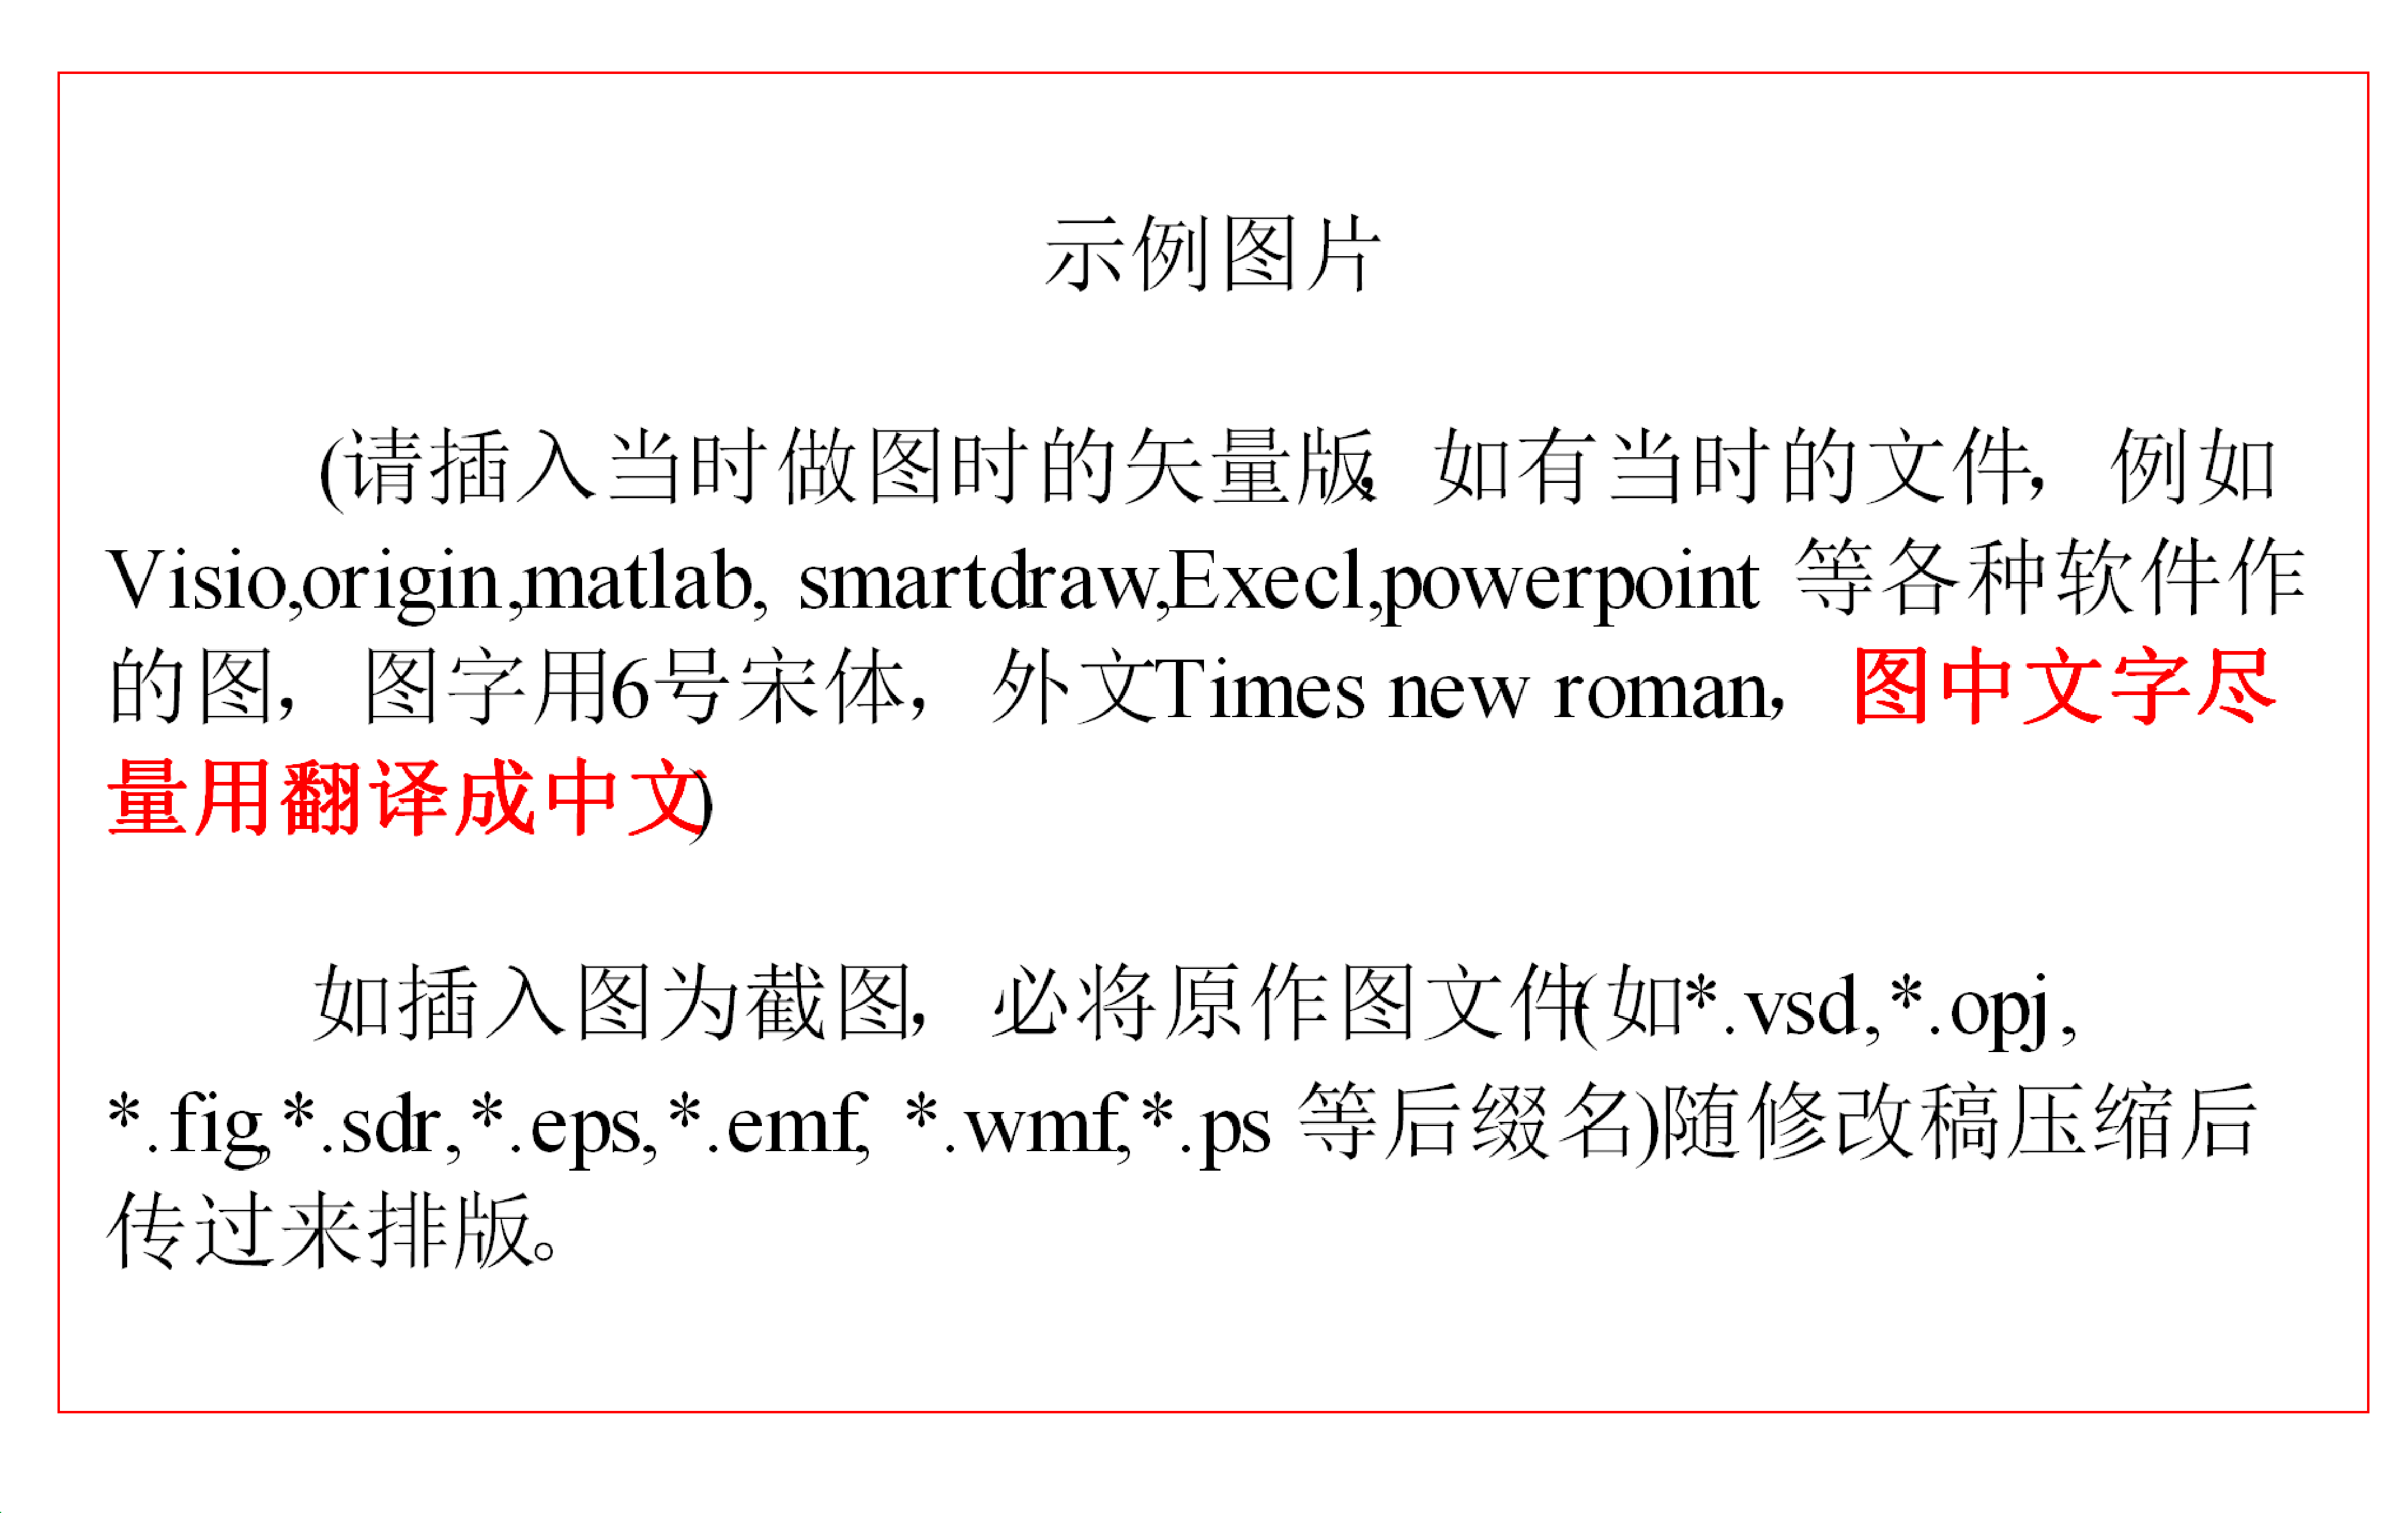
\includegraphics[width=3.15in,height=1.98in]{CJC1.pdf}}
ͼX\quad  ͼƬ˵Ã÷ *×ÖÌåΪС5ºÅ£¬Í¼Æ¬Ó¦ÎªºÚ°×ͼ£¬Í¼ÖеÄ×ÓͼҪÓÐ×Óͼ˵Ã÷*
\label{fig1}
\end{figure}

\begin{table}[htbp]
\centering {\begin{CJK*}{GBK}{hei}±íX\quad ±í˵Ã÷ *±í˵Ã÷²ÉÓúÚÌå*\end{CJK*}}
\vspace {-2.5mm}
\begin{center}
\begin{tabular}{ll}
\toprule
*ʾÀý±í¸ñ*&*µÚ1ÐÐΪ±íÍ·,±íÍ·ÒªÓÐÄÚÈÝ* \\
\hline
&
 \\
&
 \\
&
 \\
&
 \\
\bottomrule
\end{tabular}
\label{tab1}
\end{center}
\end{table}

\begin{CJK*}{GBK}{hei}¹ý³ÌX.\end{CJK*}\quad ¹ý³ÌÃû³Æ

{\zihao{5-}*¡¶¼ÆËã»úѧ±¨¡·µÄ·½·¨¹ý³ÌÃèÊö×ÖÌåΪС5ºÅËÎÌ壬IF¡¢THENµÈα´úÂë¹Ø¼ü´ÊÈ«²¿Óôóд×Öĸ£¬±äÁ¿ºÍº¯ÊýÃû³ÆÓÃбÌå*}


\begin{CJK*}{GBK}{hei}Ëã·¨\textbf{Y}\end{CJK*}.\quad Ëã·¨Ãû³Æ.
\zihao{5-}{

\noindent ÊäÈ룺{\ldots} {\ldots}

\noindent Êä³ö£º{\ldots} {\ldots}

*¡¶¼ÆËã»úѧ±¨¡·µÄËã·¨ÃèÊö×ÖÌåΪС5ºÅËÎÌå, IF¡¢THENµÈα´úÂë¹Ø¼ü´ÊÈ«²¿Óôóд×Öĸ£¬±äÁ¿ºÍº¯ÊýÃû³ÆÓÃбÌå*}

\vspace {3mm}
\zihao{5}{
\noindent \begin{CJK*}{GBK}{hei}ÖÂ\quad л\end{CJK*}\quad \begin{CJK*}{GBK}{kai} *ÖÂлÄÚÈÝ.* ÖÂл\end{CJK*}}


\vspace {5mm}
\centerline
{\zihao{5}
\begin{CJK*}{GBK}{hei}²Î~¿¼~ÎÄ~Ï×\end{CJK*}}

\begin{thebibliography}{99}
\zihao{5-} \addtolength{\itemsep}{-1em}
\vspace {1.5mm}

\bibitem[1]{1}
ÍøÉϵÄÎÄÏ×(¾ÙÀý£ºThe Cooperative
Association for Internet Data Analysis(CAIDA),http://www.caida.org/data
2010,7,18) \textbf{*Çë²ÉÓýÅ×¢·ÅÓÚÕýÎijöÏÖ´¦£¬Ã¿Ò³µÄ½Å×¢´Ó1¿ªÊ¼±àÐòºÅ*}\footnote{The Cooperative Association for Internet Data
Analysis (CAIDA), http://www.caida.org/data 2010, 7, 18}

\bibitem[2]{2} ÖÐÎĵIJο¼ÎÄÏ×Ðè¸ø³öÖÐÓ¢ÎĶÔÕÕ¡£ÐÎʽÈç[3]¡£

\bibitem[3]{3} Zhou Yong-Bin, Feng Deng-Guo. Design and analysis of cryptographic
protocols for RFID. Chinese Journal of Computers, 2006, 29(4): 581-589 (in
Chinese) \newline
(ÖÜÓÀ±ò, ·ëµÇ¹ú. RFID°²È«Ð­ÒéµÄÉè¼ÆÓë·ÖÎö. ¼ÆËã»úѧ±¨, 2006, 29(4): 581-589)

\bibitem[4]{4} ÆÚ¿¯¡¢»áÒé¡¢Êé¼®Ãû³Æ²»ÄÜÓÃËõд¡£

\bibitem[5]{5} ×÷Õß(Íâ¹úÈËÐÕÔÚÇ°£¬ÃûÔÚºó¿ÉËõд, ºóͬ).
ÌâÄ¿(Ó¢ÎÄÌâÄ¿µÚÒ»×Öĸ´óд£¬ÆäËü¾ùСд)£º¸±±êÌâ(Èç¹ûÓÐ). ¿¯Ãû(È«³Æ), Äê,
¾í(ÆÚ): Ò³Âë \textbf{*ÆÚ¿¯ÂÛÎĸñʽ*}

\bibitem[6]{6}×÷Õß.
ÎÄÕÂÌâÄ¿(Ó¢ÎÄÌâÄ¿µÚ1×Öĸ´óд£¬ÆäËü¾ùСд)£º¸±±êÌâ(Èç¹ûÓÐ)//Proceedings of
the {\ldots} (»áÒéÃû³Æ). »áÒéÕÙ¿ª³ÇÊÐ, »áÒéÕÙ¿ª³ÇÊÐËùÔÚ¹ú¼Ò, Äê: Ò³Âë
\textbf{*»áÒéÂÛÎļ¯ÂÛÎĸñʽ*}

\bibitem[7]{7}×÷Õß. ÎÄÕÂÌâÄ¿(Ó¢ÎÄÌâÄ¿µÚÒ»×Öĸ´óд, ÆäËü¾ùСд):
¸±±êÌâ(Èç¹ûÓÐ)//±àÕß. Îļ¯±êÌâ. ³ö°æµØ: ³ö°æÉç, ³ö°æÄê: Ò³Âë
\textbf{*Îļ¯¸ñʽ*}

\bibitem[8]{8}×÷Õß. ÊéÃû: ¸±±êÌâ(Èç¹ûÓÐ). °æ´Î(³õ°æ²»Ð´). ³ö°æÉçµØµã: ³ö°æÉç,
³ö°æÄê \textbf{*Êé¼®¸ñʽ*}

\bibitem[9]{9}×÷Õß. ÎÄÕÂÌâÄ¿[²©Ê¿Ñ§Î»ÂÛÎÄ/˶ʿѧλÂÛÎÄ]. µ¥Î»Ãû³Æ,µ¥Î»µØµã, Äê
\textbf{*ѧλÂÛÎĸñʽ*}

\bibitem[10]{10}×÷Õß. ÎÄÕÂÌâÄ¿(Ó¢ÎÄÌâÄ¿µÚÒ»×Öĸ´óд£¬ÆäËü¾ùСд). µ¥Î»µØµã: µ¥Î»,
¼¼Êõ±¨¸æ: ±¨¸æ±àºÅ, Äê \textbf{*¼¼Êõ±¨¸æ*}

\bibitem[11]{11}רÀûÓµÓÐÈË. רÀûÃû³Æ£¬×¨ÀûÊÚȨ¹ú¼Ò£¬×¨ÀûÊÚȨÈÕÆÚ
\textbf{*¼¼ÊõרÀû*}
  \end{thebibliography}

\begin{strip}
\end{strip}

\noindent {\zihao{5}\bf{¸½Â¼X}.}

{\zihao{5-}\setlength\parindent{2em}
*\textbf{¸½Â¼ÄÚÈÝ}ÖÃÓÚ´Ë´¦£¬×ÖÌåΪС5ºÅËÎÌå¡£¸½Â¼ÄÚÈÝ°üÀ¨£º\textbf{ÏêϸµÄ¶¨ÀíÖ¤Ã÷¡¢¹«Ê½ÍƵ¼¡¢Ô­Ê¼Êý¾Ý}µÈ*}

\begin{strip}
\end{strip}

\begin{biography}[yourphotofilename.jpg]
\noindent
\textbf{First A. Author}\ \ *¼ÆËã»úѧ±¨µÚ1×÷ÕßÌṩÕÕƬµç×ÓͼƬ£¬³ß´çΪ1´ç¡£Ó¢ÎÄ×÷Õß½éÉÜÄÚÈÝ°üÀ¨£º³öÉúÄê,ѧλ(»òĿǰѧÀú),Ö°³Æ,Ö÷ÒªÑо¿ÁìÓò(\textbf{ÓëÖÐÎÄ×÷Õß½éÉÜÖеÄÑо¿·½ÏòÒ»ÖÂ}).*
*×ÖÌåΪС5ºÅTimes New Roman*

\end{biography}

\begin{biography}[yourphotofilename.jpg]
\noindent
\textbf{Second B. Author} *Ó¢ÎÄ×÷Õß½éÉÜÄÚÈÝ°üÀ¨£º³öÉúÄê,ѧλ(»òĿǰѧÀú),Ö°³Æ,Ö÷ÒªÑо¿ÁìÓò(\textbf{ÓëÖÐÎÄ×÷Õß½éÉÜÖеÄÑо¿·½ÏòÒ»ÖÂ})¡£*
*×ÖÌåΪС5ºÅTimes New Roman*
\end{biography}
\begin{strip}
\end{strip}
\zihao{5}
\noindent \textbf{Background}

\zihao{5-}{
\setlength\parindent{2em}
*ÂÛÎı³¾°½éÉÜΪ\textbf{Ó¢ÎÄ}£¬×ÖÌåΪС5ºÅTimes New RomanÌå*

ÂÛÎĺóÃæΪ400µ¥´Ê×óÓÒµÄÓ¢Îı³¾°½éÉÜ¡£½éÉܵÄÄÚÈÝ°üÀ¨£º

±¾ÎÄÑо¿µÄÎÊÌâÊôÓÚÄÄÒ»¸öÁìÓòµÄʲôÎÊÌâ¡£¸ÃÀàÎÊÌâÄ¿Ç°¹ú¼ÊÉϽâ¾öµ½Ê²Ã´³Ì¶È¡£

±¾ÎĽ«ÎÊÌâ½â¾öµ½Ê²Ã´³Ì¶È¡£

¿ÎÌâËùÊôµÄÏîÄ¿¡£

ÏîÄ¿µÄÒâÒå¡£

±¾Ñо¿ÈºÌåÒÔÍùÔÚÕâ¸ö·½ÏòÉϵÄÑо¿³É¹û¡£

±¾ÎĵijɹûÊǽâ¾ö´ó¿ÎÌâÖеÄÄÄÒ»²¿·Ö£¬Èç¹ûÉæ¼°863$\backslash
$973ÒÔ¼°ÆäÏîÄ¿¡¢»ù½ð¡¢Ñо¿¼Æ»®£¬×¢ÒâÕâЩÏîÄ¿µÄÓ¢ÎÄÃû³ÆÓ¦ÊéдÕýÈ·¡£}

\end{CJK*}
\end{document}


